\section{Blink}

Für die Blink Entity-Architecture wurden sämtliche bisher angefertigte Entity-Architectures angewandt:

\begin{center}
    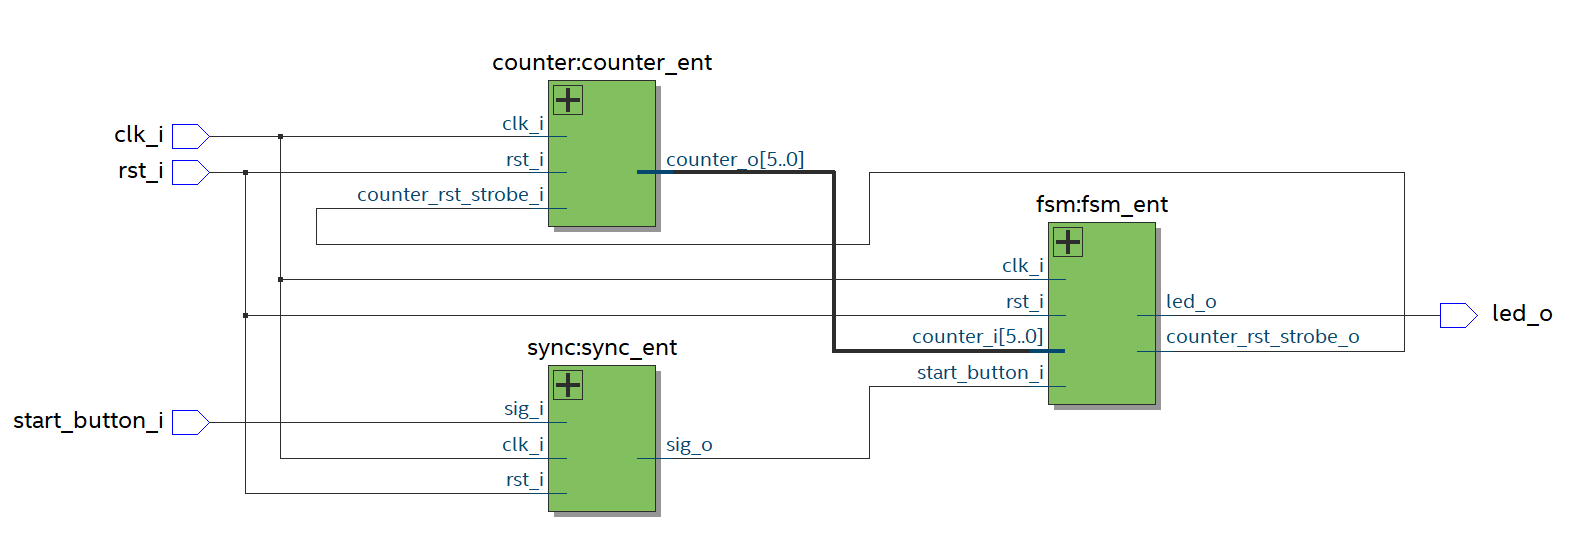
\includegraphics[width=1\linewidth]{images/BlinkBSB.png}
\end{center}

Counter und FSM Entities werden hier nur kurz als Blockschaltbild gezeigt, da diese bereits in vergangenen Übungen aufgekommen sind. Natürlich wurde auch das Feedback berücksichtigt und dementsprechend Verbesserungen vorgenommen.

\subsection{Counter} 

\begin{center}
    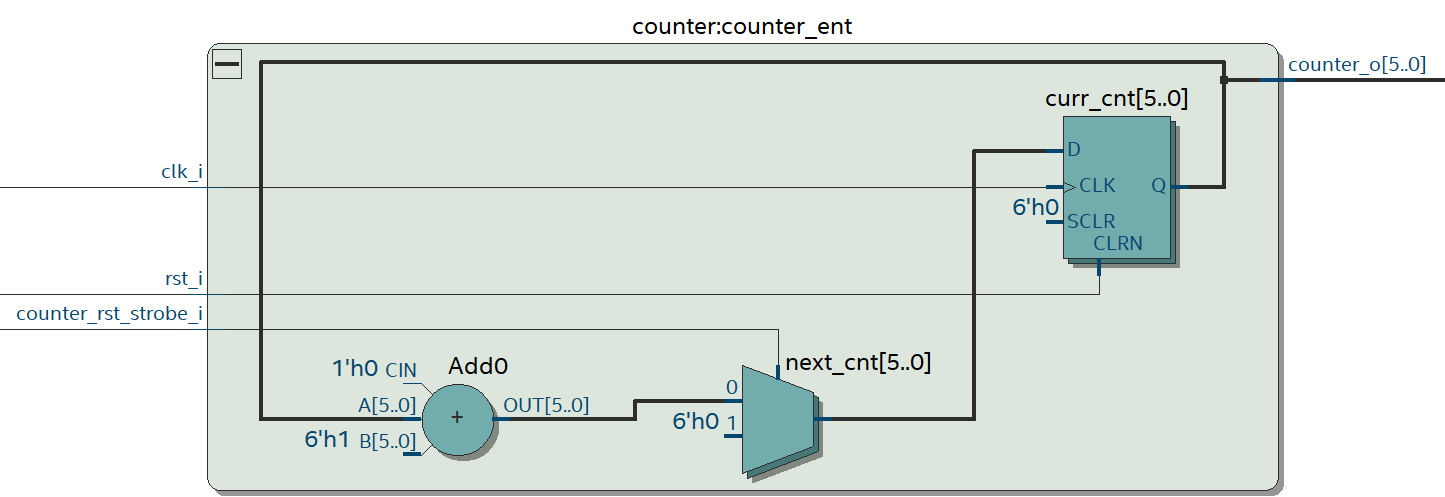
\includegraphics[width=0.75\linewidth]{images/CounterBSB.png}
\end{center}

\begin{quote}
\end{quote}

\subsection{Finite-State-Machine}

\begin{center}
    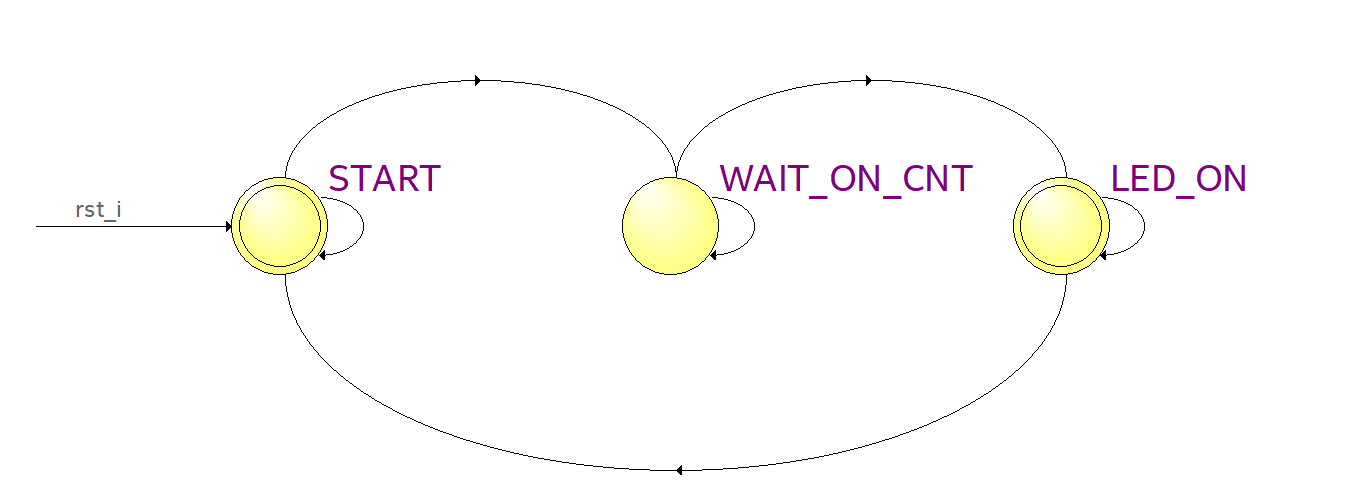
\includegraphics[width=0.5\linewidth]{images/fsm.png}
\end{center}

\begin{quote}
\end{quote}

\newpage

\subsection{Synchronizer Chain}

\begin{center}
    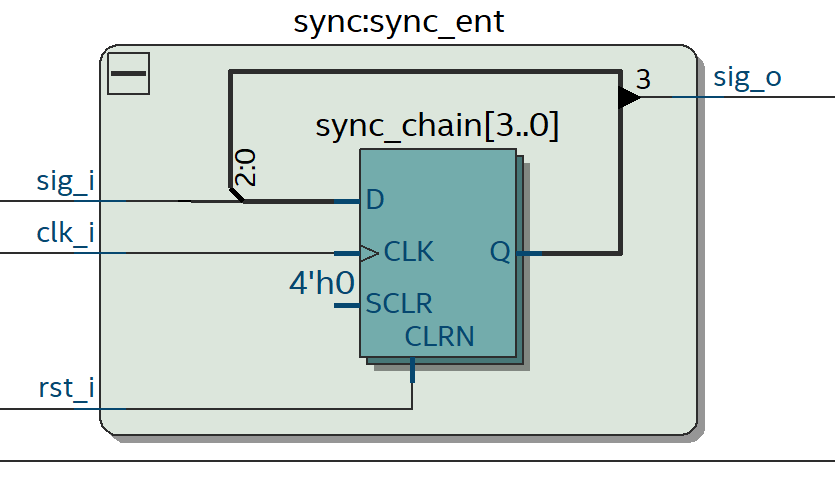
\includegraphics[width=0.5\linewidth]{images/SyncBSB.png}
\end{center}

\textbf{Entity}\hrulefill

\begin{lstlisting}
entity sync is
    generic (
        N_DFF : natural := 1
    );
    port (
        clk_i : in std_ulogic;
        rst_i : in std_ulogic;
        sig_i : in std_ulogic;
        sig_o : out std_ulogic
    );
end sync;
\end{lstlisting} 

\textbf{Architecture}\hrulefill

Signale

\begin{lstlisting}
signal sync_chain : std_logic_vector(N_DFF-1 downto 0) := (others => '0');
signal next_sync_chain : std_logic_vector(N_DFF-1 downto 0) := (others => '0');
\end{lstlisting}

(1) \lstinline{reg_seq : process (clk_i, rst_i)} 

\begin{quote}
Weist bei einem Reset dem gesamten \lstinline{sync_chain} Vektor \lstinline{'0'} zu. Bei der steigenden Flanke wird diesem Vektor ein kombinatorisch ermittelter Vektor \lstinline{next_sync_chain} zugewiesen.
\end{quote}

(2) \lstinline{comb : process (sig_i, sync_chain)}

\begin{quote}
Der Eingang \lstinline{sig_i} geht in den ersten Slot des \lstinline{next_sync_chain} Vektors über. Danach wird jeweils der vorherige \lstinline{sync_chain} Wert mit der nächste Stelle des \lstinline{next_sync_chain} Vektors verbunden.
\end{quote}

Der Ausgang dieses Systems ist der letzte Wert im \lstinline{sync_chain} Vektor.

\textbf{Simulation}\hrulefill

\begin{center}
    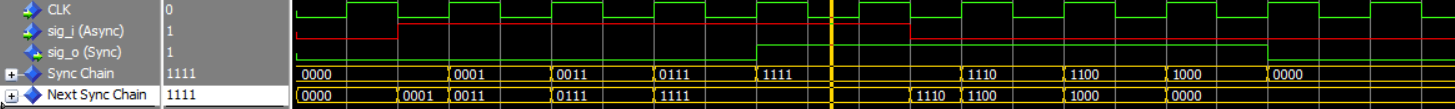
\includegraphics[width=1\linewidth]{images/SyncSim.png}
\end{center}

\newpage

\subsection*{Simulation}

\begin{center}
    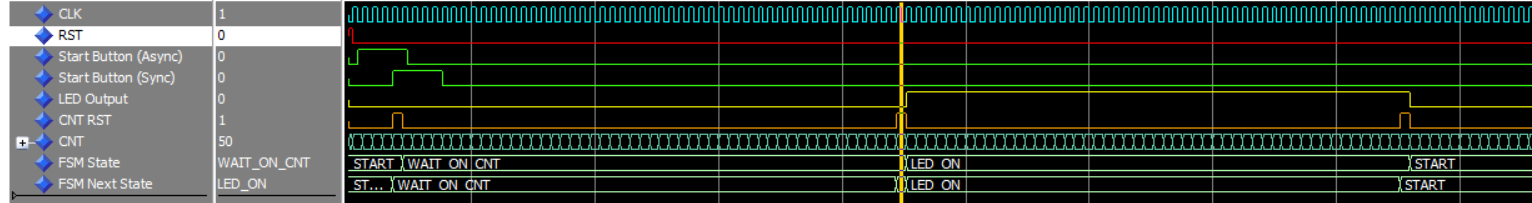
\includegraphics[width=1\linewidth]{images/BlinkSim.png}
\end{center}


